\documentclass[a4paper]{article}
\usepackage[utf8]{inputenc} % Skal passe til editorens indstillinger
\usepackage[english]{babel} % danske overskrifter


\newcommand{\name}{Carsten Nielsen}
%\newcommand{\stnumber}{s123369, s123161, s123821}
\newcommand{\course}{INI 404 Neuromorphic Engineering~I}
\newcommand{\university}{University of Zürich}
\newcommand{\studyline}{Institute of Neuroinformatics}
\newcommand{\assignment}{Lab 8 Post-Lab}
\renewcommand{\date}{\today} %If another date, than that of today is desiered


% Palatino for rm and math | Helvetica for ss | Courier for tt
\usepackage{mathpazo} % math & rm
\linespread{1.05}        % Palatino needs more leading (space between lines)
\usepackage{palatino} % tt
\normalfont
\usepackage[T1]{fontenc}
\usepackage[english]{babel}

\usepackage{graphicx}%allerese hentet % indsættelse af billeder
\usepackage{epstopdf} %Tilfj "--enable-write18" i argumentet for LaTex build. Dette vil konvertere .eps figurer til pdf-format
\graphicspath{{./picture/}} % stivej til bibliotek med figurer
\usepackage{subcaption} %Til gruppering af figurer
\usepackage{amsmath} %matpakke
\usepackage{amsfonts} %
\usepackage{amssymb} %
\usepackage{steinmetz} % flere matematik symboler
\usepackage{polynom} %for displaying polynom division
\usepackage{mathtools} % matematik - understøtter muligheden for at bruge \eqref{}
\usepackage{float}
\usepackage{placeins}
\usepackage{hhline}

%
\usepackage[usenames,dvipsnames]{xcolor}
\usepackage[compact,explicit]{titlesec}% http://ctan.org/pkg/titlesec
%
\usepackage[europeanresistors]{circuitikz}
\usepackage{pgfplots}
\usepgfplotslibrary{patchplots}
\pgfplotsset{compat=1.11}

%---------%
%Easy edit%
%---------%

%Section formating. arg1 is supplied when making section
\newcommand\presectionnumber[1]{~~}
\newcommand\postsectionnumber[1]{}
\newcommand\midlesection[1]{#1}
\newcommand\sectionnum[1]{\arabic{#1}}
\newcommand\subsectionnum[1]{\arabic{#1}}
\newcommand\subsubsectionnum[1]{\alph{#1}}



%------------%
%setion setup%
%------------%
\renewcommand\thesection{Opgave~\sectionnum{section}} %pas p�, kun i matematik
\renewcommand\thesubsection{\thesection,~\subsectionnum{subsection}}
\definecolor{MagRed}{RGB}{190,40,15}
\definecolor{MathGreen}{RGB}{82,164,0}

\titleformat{\section}{\normalfont\sffamily\large\bfseries\color{MathGreen}}{}{0pt}{|\kern-0.15ex|\kern-0.15ex|\kern-0.15ex|\presectionnumber{#1}\sectionnum{section}\postsectionnumber{#1}\qquad\quad\midlesection{#1}\label{sec:\sectionnum{section}}}
\titleformat{\subsection}[runin]{\large\bfseries}{}{10pt}{\sectionnum{section}.\subsectionnum{subsection})~#1\label{sec:\sectionnum{section}.\subsectionnum{subsection}}}
\titleformat{\subsubsection}[runin]{\itshape}{}{0pt}{\subsectionnum{subsection},\subsubsectionnum{subsection}~#1\label{sec:\sectionnum{section}.\subsectionnum{subsection}.\subsubsectionnum{subsubsection}}}
%\titleformat{\subsubsection}{\bfseries}{}{0pt}{\alph{subsection}.\arabic{subsubsection})\qquad\quad#1\label{\arabic{section}\alph{subsection}\arabic{subsubsection}}}

%----------%
%page setup%
%----------%
\textwidth = 400pt
\marginparwidth = 86pt
\hoffset = -25pt
\voffset= -30pt
\textheight = 670pt

%--------%
%hyperref%
%--------%
\newcommand{\HRule}{\rule{\linewidth}{0.5mm}}
\usepackage{fancyhdr}
\usepackage[plainpages=false,pdfpagelabels,pageanchor=false]{hyperref} % aktive links
\hypersetup{%
  pdfauthor={\name},
  pdftitle={\assignment},
  pdfsubject={\course} }
%\usepackage{memhfixc}% rettelser til hyperref

%-------------%
%Headder setup%
%-------------%
\fancyhf{} % tom header/footer
\fancyhfoffset{20pt}
\fancyhfoffset{20pt}
\fancyhead[OL]{\name \\ INI 404}
\fancyhead[OC]{Date \\ \date}
\fancyhead[OR]{\university\\ \studyline}
\fancyfoot[FL]{}
\fancyfoot[FC]{\thepage}
\fancyfoot[FR]{}
\renewcommand{\headrulewidth}{0.4pt}
\renewcommand{\footrulewidth}{0.4pt}
\headsep = 35pt
\pagestyle{fancy}
 % style setup

%Listings%
\usepackage{listingsutf8}
\usepackage[framed,numbered]{matlab-prettifier}


%setup listings
\lstset{language=Matlab,
  extendedchars=true,
  language=Octave,                % the language of the code
  basicstyle=\ttfamily\footnotesize,           % the size of the fonts that are
  % used for the code
  numbers=left,                   % where to put the line-numbers
  numberstyle=\tiny\color{gray},  % the style that is used for the line-numbers
  stepnumber=2,                   % the step between two line-numbers. If it's 1, each line 
                                  % will be numbered
  numbersep=5pt,                  % how far the line-numbers are from the code
  backgroundcolor=\color{white},      % choose the background color. You must add \usepackage{color}
  showspaces=false,               % show spaces adding particular underscores
  showstringspaces=false,         % underline spaces within strings
  showtabs=false,                 % show tabs within strings adding particular underscores
  frame=single,                   % adds a frame around the code
  rulecolor=\color{black},        % if not set, the frame-color may be changed on line-breaks within not-black text (e.g. comments (green here))
  tabsize=4,                      % sets default tabsize to 2 spaces
  captionpos=b,                   % sets the caption-position to bottom
  breaklines=true,                % sets automatic line breaking
  breakatwhitespace=false,        % sets if automatic breaks should only happen at whitespace
  title=\lstname,                   % show the filename of files included with \lstinputlisting;
                                  % also try caption instead of title
  %keywordstyle=\color{blue},          % keyword style
  %commentstyle=\color{dkgreen},       % comment style
  %stringstyle=\color{mauve},         % string literal style
  escapeinside={\%*}{*)},            % if you want to add LaTeX within your code
  morekeywords={*,...},              % if you want to add more keywords to the set
  deletekeywords={...}              % if you want to delete keywords from the given language
}
\lstset{literate=
  {á}{{\'a}}1 {é}{{\'e}}1 {í}{{\'i}}1 {ó}{{\'o}}1 {ú}{{\'u}}1
  {Á}{{\'A}}1 {É}{{\'E}}1 {Í}{{\'I}}1 {Ó}{{\'O}}1 {Ú}{{\'U}}1
  {à}{{\`a}}1 {è}{{\`e}}1 {ì}{{\`i}}1 {ò}{{\`o}}1 {ù}{{\`u}}1
  {À}{{\`A}}1 {È}{{\'E}}1 {Ì}{{\`I}}1 {Ò}{{\`O}}1 {Ù}{{\`U}}1
  {ä}{{\"a}}1 {ë}{{\"e}}1 {ï}{{\"i}}1 {ö}{{\"o}}1 {ü}{{\"u}}1
  {Ä}{{\"A}}1 {Ë}{{\"E}}1 {Ï}{{\"I}}1 {Ö}{{\"O}}1 {Ü}{{\"U}}1
  {â}{{\^a}}1 {ê}{{\^e}}1 {î}{{\^i}}1 {ô}{{\^o}}1 {û}{{\^u}}1
  {Â}{{\^A}}1 {Ê}{{\^E}}1 {Î}{{\^I}}1 {Ô}{{\^O}}1 {Û}{{\^U}}1
  {œ}{{\oe}}1 {Œ}{{\OE}}1 {æ}{{\ae}}1 {Æ}{{\AE}}1 {ß}{{\ss}}1
  {ç}{{\c c}}1 {Ç}{{\c C}}1 {ø}{{\o}}1 {å}{{\r a}}1 {Å}{{\r A}}1
  {€}{{\EUR}}1 {£}{{\pounds}}1
}

 \lstloadlanguages{% Check Dokumentation for further languages ...
         %[Visual]Basic
         %Pascal
         %C
         %C++
         %XML
         %HTML
         %Java
         %VHDL
         Matlab
 }
 %Listings slut%









%Matematik hurtige ting
%fed
\renewcommand\vec[1]{\mathbf{#1}}
\newcommand\matr[3]{{}_{#2}\mathbf{#1}{}_{#3}}
\newcommand\facit[1]{\underline{\underline{#1}}}
%\renewcommand\d[3]{\frac{\mbox{d}^{#3}#1(#2)}{\mbox{d}#2^{#3}}}
%underline
%\renewcommand\vec[1]{\underline{#1}}
%\newcommand\matr[3]{{}_{#2}\underline{\underline{#1}}{}_{#3}}

\renewcommand\matrix[4]{ %{alignment}{to space}{from space}{matrix}
{\vphantom{\left[\begin{array}{#1}#4\end{array}\right]}}_{#2}\kern-0.5ex
\left[\begin{array}{#1}
#4
\end{array}\right]_{#3}
}
\newcommand\e[0]{\mbox{e}}
\newcommand\E[1]{\cdot 10^{#1}}
\newcommand\im[0]{i}

\newcommand\Jaco{\mbox{Jacobi}}
\newcommand\del[2]{\frac{\partial {#1}}{\partial {#2}}}
\newcommand\abs[1]{\left| {#1} \right|}
\newcommand\stdfig[4]{ %width,img,cap,lab
\begin{figure}[H]
\centering
\includegraphics[width={#1}\textwidth]{#2}
\caption{#3}
\label{#4}
\end{figure}
}
\newcommand\stdfignoscale[3]{ %img,cap,lab
\begin{figure}[H]
\centering
\includegraphics{#1}
\caption{#2}
\label{#3}
\end{figure}
}
\newcommand\diff{\dot}
\newcommand\ddiff{\ddot}
\newcommand\dddiff{\dddot}
\newcommand\ddddiff{\ddddot}






% How to make ref to books or urls in bib
%\citetitle[fx: page 1]{name of ref in bib}


\tikzset{rrail/.style={rground,yscale=-1}}
\newcommand{\reffig}[1]{Fig.~\ref{#1}}

\begin{document}
\begin{titlepage}
\centering \parindent=0pt

\vspace*{\stretch{1}} \HRule\\[1cm]\Huge
\course\\[0.7cm]
\large \assignment\\[1cm]
\HRule\\[4cm]  
%\includegraphics[width=6cm]{picture}\\ Use this if you want a picture on the frontpage
\name\\
%\stnumber
TAs: Ning Quiao, Chenghan Li

\vspace*{\stretch{2}} \normalsize %

\begin{center}
	\date 
\end{center}
\vspace*{\stretch{2}} \normalsize
\begin{flushright}
%\includegraphics[width=6cm]{./dtu.eps}\\
\end{flushright}
\end{titlepage}

\newpage

\section{Adaptive Photoreceptor Gain}

In this experiment we measured the small signal characteristics of the adaptive photoreceptor and of the non-adapting photoreceptor for comparison. In order to get different DC values of light, we used two filters, the attenuation of the second one being 100 times that of the first. The results of applying a square input wave can be seen in Fig.~\ref{fig:exp1}.

\begin{figure}[H]
	 \center
	 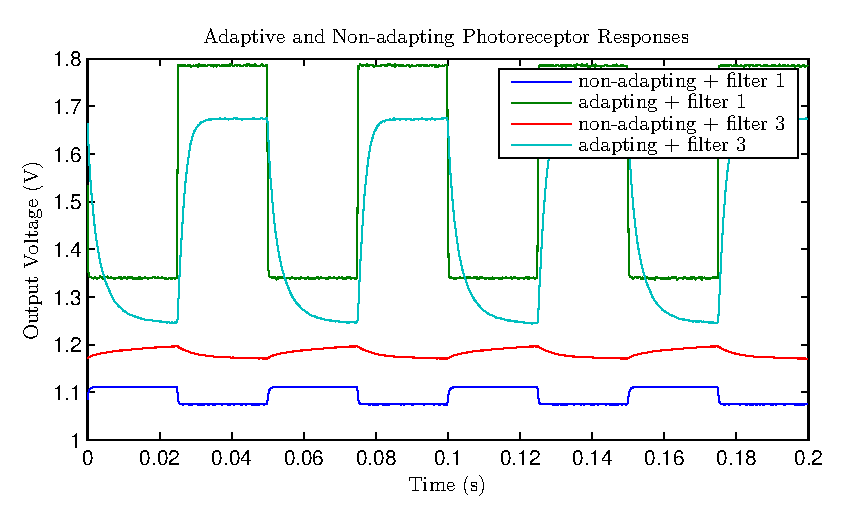
\includegraphics{exp1.eps}
	 \caption{Responses of the adaptive and non-adapting photoreceptor circuits to two square small signals of light with different offsets.}
	 \label{fig:exp1}
\end{figure}
We can observe that the adaptive photoreceptor is faster than the non-adapting due to the positive feedback. 

When the DC value of the light signal is smaller (filter 3), the responses are slower. We can also see that, in this case, the gain of the non-adapting photoreceptor decreases but the gain of the adaptive photoreceptor remains constant as expected. \\ 


\subsection{Extra credit: Loop gain}
We measured the amplitude of the signal at the photodiode node and found it to be \(V_{in}=3.6\cdot10^{-3}\) while the amplitude at the output was \(V_{out}=0.44\). From this we can calculate the gain of the amplifier as \(A_{amp}=\frac{V_{out}}{V_{in}}=120\).
The amplitude of the signal at the feedback node was \(V_{fb}=0.055\), so the capacitive divider is \(A_C=\frac{V_{fb}}{V_{out}}=0.13\). 
Assuming $\kappa$ to be 0.8, the total loop gain is given by

\begin{equation*}
A_{loop}=A_{amp} \cdot A_c \cdot \kappa = 12
\end{equation*}
	\\
\section{Photoreceptor Time Response}
\subsection{Adaptation time-constants}
Here we investigate how fast the photoreceptor adapts to a big change in illumination. For this, we use a 0.1 Hz and 2 V signal. The results can be seen in  Fig.~\ref{fig:exp2.1}.

\begin{figure}[H]
	\center
	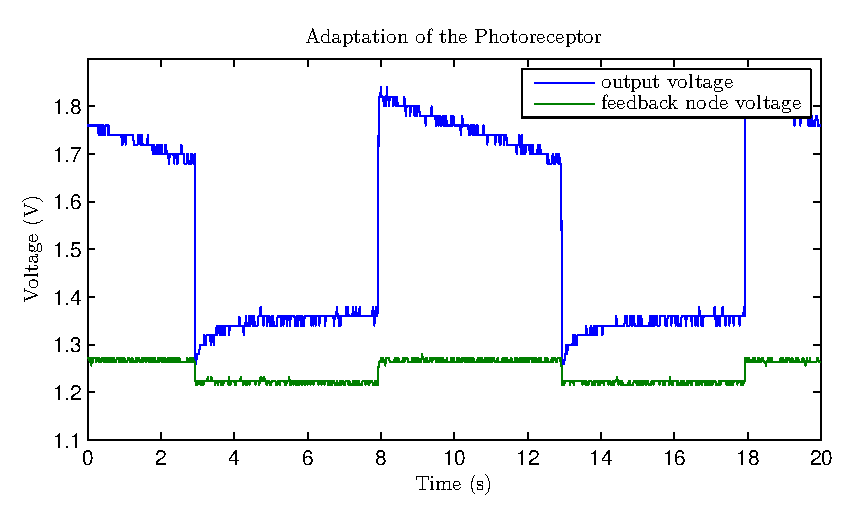
\includegraphics{exp2_1.eps}
	\caption{Output and feedback node of the adaptive photoreceptor using a square large signal of light as input.}
	\label{fig:exp2.1}
\end{figure}

The photoreceptor adapts more quickly to negative steps, the adaptation time being approximately 1 second. For positive steps, the adaptation time is larger than 2.5.\\ 

\subsection{Effect of illumination on the response time and using the cascode to increase the bandwith}
In this experiment, we measure how the bandwidth (1/(rise time)) scales with DC illumination and how the cascode can be used to increase the bandwidth.
\begin{figure}[H]
	\center
	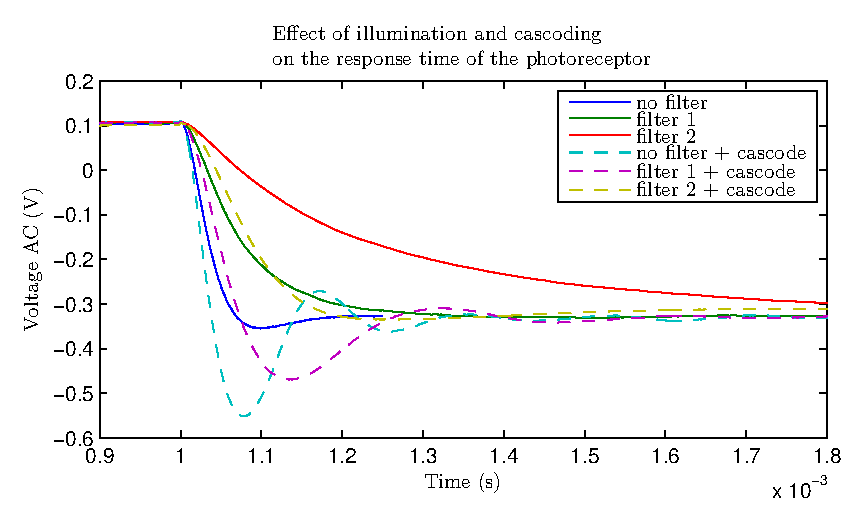
\includegraphics{exp2_2a.eps}
	\caption{Response of the adaptive photoreceptor to a small step in input light for three different offset values with and without using the cascode ($V_c=2$ or 5 respectively).}
	\label{fig:exp2.2a}
\end{figure}

\begin{figure}
	\center
	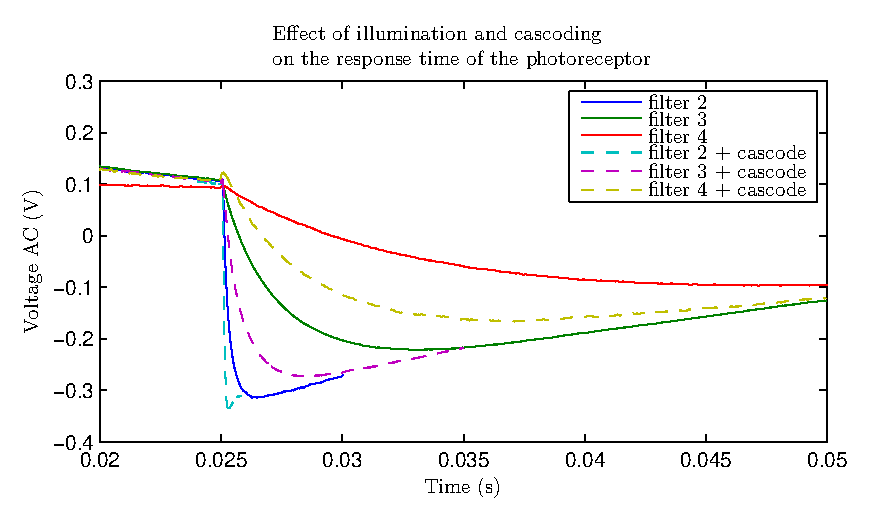
\includegraphics{exp2_2b.eps}
	\caption{Response of the adaptive photoreceptor to a small step in input light for three different offset values with and without using the cascode ($V_c=2$ or 5 respectively). The values corresponding to the highest offset value (filter 2) are repeated for comparison with Fig.~\ref{fig:exp2.2a}.} 
	\label{fig:exp2.2b}
\end{figure}

\begin{figure}[H]
	\center
	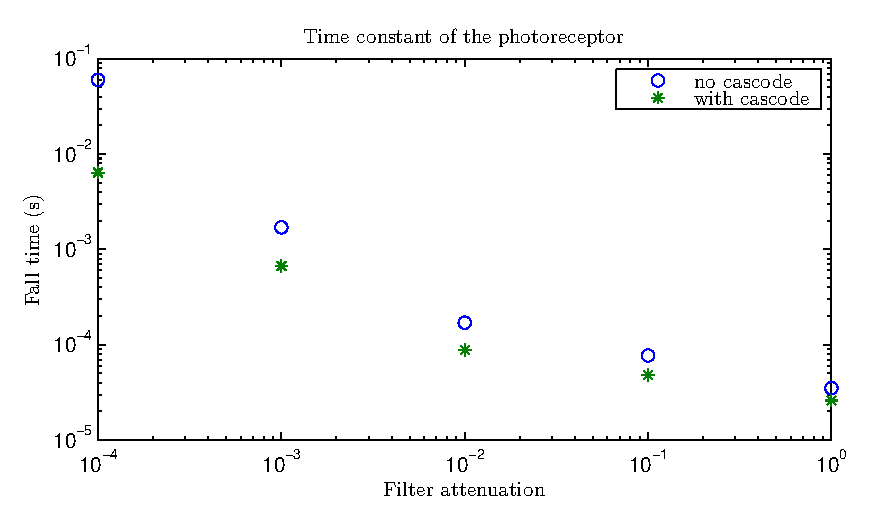
\includegraphics{exp2_2c.eps}
	\caption{Time constants of the adaptive photoreceptor for different offset values with and without using the cascode as measured from Fig.~\ref{fig:exp2.2a} and Fig.~\ref{fig:exp2.2b}.}
	\label{fig:exp2.2c}
\end{figure}

Figures \ref{fig:exp2.2a} and \ref{fig:exp2.2b} show the responses of the circuit to a small negative step in illumination using different filters to get five different DC values. The time constants measured from these experiments are displayed in Fig.~\ref{fig:exp2.2c} on logarithmic scale. 

The use of the cascode makes the response of the circuit faster (although of the same order of magnitude) but it introduces overshoot for high DC illumination values. 

The time constants are inversely proportional to the current through the photodiode so they should decrease exponentially with increasing illumination. This seems to be true for some ranges of illumination but there appears to be a change in behavior around the 100 attenuation point. \\

\subsection{Extra credit: The tobi element}
Lastly, we measure the I-V characteristic of the tobi element applying voltages and measuring the generated current. The results are shown in Fig.~\ref{fig:tobi} and Fig.~\ref{fig:tobilog}. For differences in voltage smaller than 4.3 V, the current from well to gate is larger than in the opposite direction. This explains why the adaptation is faster for negative steps, where current has to flow into the capacitor through the tobi element from well to gate.

\begin{figure}[H]
	\center
	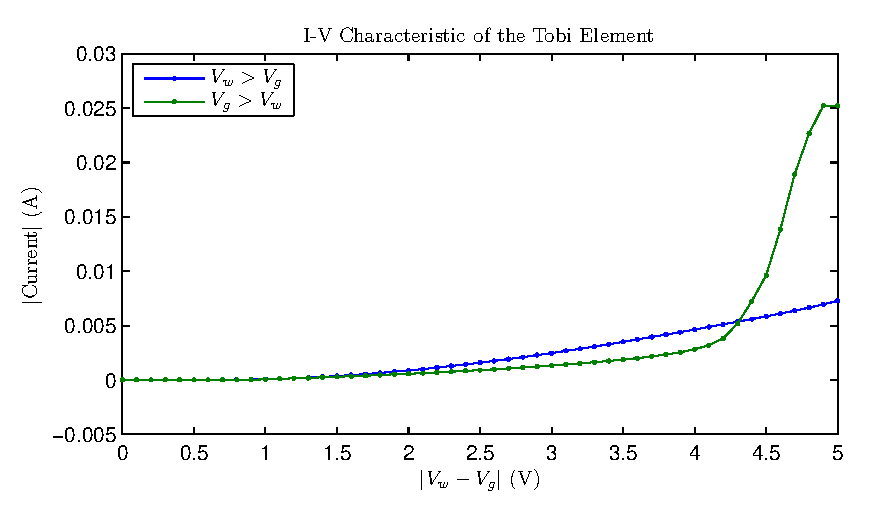
\includegraphics{tobi.eps}
	\caption{I-V curve of the tobi element. To make the comparison between forward and reverse current more clear, we have plotted the absolute values of current and voltage.}
	\label{fig:tobi}
\end{figure}

\begin{figure}
	\center
	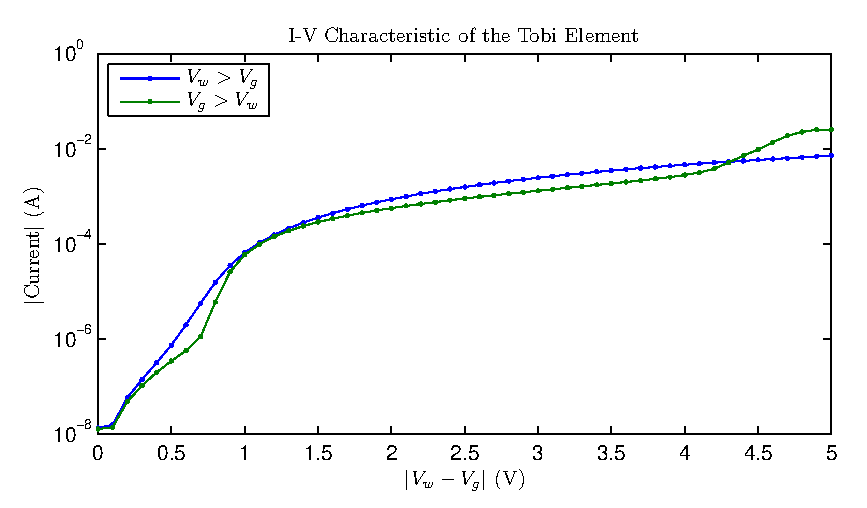
\includegraphics{tobilog.eps}
	\caption{I-V curve of the tobi element in logarithmic scale.}
	\label{fig:tobilog}
\end{figure}

\end{document}
